\documentclass[format=acmsmall, review=false, screen=true]{acmart}
\settopmatter{printacmref=false} % Removes citation information below abstract
\renewcommand\footnotetextcopyrightpermission[1]{} % removes footnote with conference information in first column
\pagestyle{plain} % removes running headers
\acmYear{2018}
\acmMonth{7}

\usepackage[utf8]{inputenc}
\usepackage{microtype}
\usepackage{amsmath}
\usepackage{listings}
\usepackage{float}
\usepackage{wrapfig}
\usepackage{subcaption}
\usepackage{dirtytalk}


\lstset{
  basicstyle=\ttfamily,
  columns=fullflexible,
  frame=single,
  breaklines=true,
  postbreak=\mbox{\textcolor{red}{$\hookrightarrow$}\space},
  aboveskip=10pt,
  belowskip=5pt,
  tabsize=2
} 

\setlength{\textfloatsep}{15pt}
\setlength{\abovecaptionskip}{6pt}
\setlength{\belowcaptionskip}{6pt}

\author{Richard Bányi}

\title{\textsc{Comparing Braintenberg vehicles evolved using classical evolutionary algorithms and neuroevolution}}
\subtitle{\textsc{IT University of Copenhagen, Summer 2018}}
\acmDOI{}
\begin{document}
\begin{abstract}
The purpose of this project is to compare different evolution strategies to the evolution and optimization of Braitenberg vehicle using classical evolutionary algorithms and neuroevolution. Braitenberg vehicles are a special class of agents that can autonomously move around based on its sensor inputs. Braitenberg vehicles are controlled by a number of parameters, depending on how the sensors and wheels are connected we can exhibit different behaviors. We show how basic evolutionary algorithms (EA’s) and neuroevolution can emulate a Braitenberg vehicle in a way that it avoids obstacles. Although the experiments will consist of a simple task of navigation and obstacle avoidance, our major goal of the project on autonomous agents is to emphasize the main differences of both approaches. V-Rep simulator will be used to test and track the evolution, however, we intend to test on a real physical agent.
	\end{abstract}
\maketitle


\section{Introduction}

Autonomous agents are characterized as intelligent agents that pursue a certain goal without external supervision or control. Take for example a self-driving car\cite{eberhard200621}, its goal is to drive from point A to point B, while ensuring the safety of its passengers, as well it has to be able to maintain its internal energy level and when its batteries are on low it drives to the nearest charging stations. In real world situation, the self-driving har has to be able to adapt to different environments, driving on the highway or on the countryside requires different behavioral capabilities. All of these features of autonomous agents are a way to complex to pre-define, and should rather emerge from the interaction between the robot and its own environment. Building an abstract pre-defined model of the world is not sufficient in a continuously changing environment. Returning back to the example of a self-driving car, putting a whole map of the environment into the vehicle is not sufficient since the environment is constantly changing, a car might encounter an unexpecting crossing pedestrian or roadblock which was not part of the abstract model. Autonomous agents are equipped with sensors and actuators. An agent perceives its environment through sensors like proximity, infrared sensors and it interacts with its environment by using actuators. 

Major steps have been already taken for building autonomous systems using classical AI approach. On one hand there is the approach termed \emph{behavior-based-robotics} from the 1980's\cite{arkin1998behavior}. Behavior-based robotics emphasize the importance of continuous interaction between the robot and its own environment for the dynamic development of the control system \cite{siciliano2016springer}. As contrasted to classical \emph{Knowledge-Based Artificial Intelligence} which is more concerned with a high level of definition of the environment. For example, the agent first sense the environment, then usually a model is built, and the robot has to reason upon this model to decide which action to take. Wahde\cite{wahde2004evolutionary} contend that this approach is very slow and could not be executed in the real world.


Beside these solutions, some other researchers have developed autonomous systems by employing various sorts of neural networks to control a robot. A  different approach is taken by researchers that try to evolve the robot control system using evolutionary algorithms. Rather than design a solution, they describe the robot characteristics in form of a chromosome. \emph{Evolutionary algorithms} \cite{back1996evolutionary} focus on global optimization problems inspired by biological evolution. EA are population-based, metaheuristic search procedures that incorporate genetic operators \cite{back1996evolutionary}. The algorithm maintains a population of candidate solutions which is subjected to natural selection and mutation. In each generation, a set of offspring is generated by applying bio operators such as \emph{mutation, crossover, selection}. Each generation, the fitness of every individual in the population is evaluated. More fit individuals are stochastically selected from the current population, and each individual's \emph{genome} is modified (recombined or randomly mutated) to form a new generation. The algorithm terminates when either the maximum number of generations has been produced, or fitness level has been reached for the population.

Within this approach, a number of researches have successfully employed an evolutionary procedure to develop a robot control system \cite{salomon1999evolving}. Although the evolutionary procedure is well known, it is not a straightforward task to apply, as discovered during implementation.

In this paper, we describe the evolution of Braitenberg like obstacle avoidance vehicle using classical evolutionary algorithm and neuroevolution. In all our experiments the evolutionary procedure is carried out in a robot simulator called V-Rep \cite{rohmer2013v}.

\section{The Robot}

In the experiments reported in this paper, the simulator (robot) was controlled through the external client. The remote API functions are interacting with V-REP (robot) via socket communication. A detailed description of V-REP and the remote API \footnote{\url{http://www.coppeliarobotics.com/helpFiles/en/remoteApiOverview.htm}} can be found online.

Pioneer P3DX was chosen for the purpose of the experiments. The robot is equipped with 16 proximity sensors and two motors. The motors can be controlled independently of each other by sending function calls to the simulator. The specifications of sensor readings and possible speed values, included normalization values are depicted in the table below \ref{fig:specs}.

\begin{table}[H]
\begin{tabular}{llll}
\hline
\textbf{}                            & \textbf{Simulator}   & \textbf{Normalized} & \textbf{Type} \\ \hline
\textbf{Speed Values}                & {[}0.0, 4.0{]}       & {[}0.0, 1.0{]}      & Float         \\
\textbf{Sensory Readings}            & {[}0.0, 1.0{]}       & {[}0.0, 1.0{]}      & Float         \\
\textbf{Detectable Object Distances} & {[}0.05, 1{]}        & {[}0.0, 1.0{]}      & Float         \\
\textbf{}                            & \textbf{No readings} & \textbf{Close}      & \textbf{Far}  \\
\textbf{Sensory Readings}            & 0.0                  & 0.1                 & 0.9          
\end{tabular}
\caption{Sensors and speed values specification}
\label{fig:specs}
\end{table}

\begin{figure}[H]
  \includegraphics[width=0.66\linewidth]{img/pioneer.PNG}
  \caption{The Pioneer P3DX robot}
  \label{fig:pioneer-robot}
\end{figure}

\section{Braitenberg Vehicles}

A Braitenberg vehicle \cite{braitenberg1986vehicles} is an agent that can autonomously move around and exhibit various different behaviors depending on its sensor inputs. The vehicle is equipped with primitive sensors that measure certain quality, and 2 motors which functions as actuators. Depending on how the sensors and motors are connected, the vehicle exhibits different behaviors. Thus the motion of the vehicle is directly controlled by the sensors. Yet the resulting behavior may appear complex or even intelligent.

Our control architecture was inspired by a Braitenberg type-2c vehicle - each sensor is connected to both motors. The sensor readings control the motors via inhibitory and excitatory connections. The key idea is that a sensor with high proximity activation accelerates the motor on the proximity sensor's side while slows down the motor on the opposite side. The presence of an obstacle leads to different motor speeds, which causes the robot to turn or spin. The activation of motors is calculated by the following formula:

\[ M_{lr} = \sum_{i=1}^{16} P_{i} w_{l_i r_i} \]

where \(P_{i}\) is the activation value of the proximity sensor \emph{i} and \(w_{lr_i}\) denotes the genome that connects proximity \(P_{i}\) with motors. In the absence of obstacle the calculation of the motor's activation is similar, however, in this case, the activation value of the proximity sensor's is left out:

\[ M_{lr} = \sum_{i=1}^{16} w_{l_i r_i} \]

\section{Experimental Setup}

\begin{figure}[H]
  \includegraphics[width=0.66\linewidth]{img/scene.PNG}
  \caption{The environment. The robot indicated position is the starting poing of every simulation as well for the fitness evaluation.}
  \label{fig:arena-scene}
\end{figure}

The robot is operating in an environment in a sort of squared corridor whose size is approximately 2x2m large in the simulator. Figure\ref{fig:arena-scene} shows the arena in which the robot has to move. In all experiments, the robot was started from an initial position which is indicated in the figure.

As already discussed, our goal was to develop a robot that could learn how to cover as much much distance as possible while avoiding obstacles on its way. In order to evolve Braitenberg like vehicles, we needed to incorporate features into our fitness function which solely relies on a set of variables that can be measured within the interaction between the robot and the environment. Hence our fitness criterion consists of two fitness classes: \emph{aggregate fitness function} and \emph{behavioral fitness function} \cite{divband2015effect}.

\emph{Aggregate fitness function} have the lowest degree of knowledge (traveled distance), and evaluate only what is achieved. In our case it relies on traveled distance. The procedure of how the robot accomplishes the task is irrelevant. The aggregate fitness function is defined by the distance that the robot traveled during the evaluation:

\[ aff = \sum_{t=1}^{t_{max}} \sqrt{(x_{previous} - x_{current})^2 + (y_{previous} - y_{current})^2} \]

On the other hand, \emph{behavioral fitness function} measures how the task is solved, hence it requires prior knowledge about options how the task can be solved. This way BFF also predetermine potential solutions and possibly exclude counterintuitive options \cite{divband2015effect}. The \emph{bff} is a function of three variables, as follows:


\[ f_{t} = V_{t} (1-\Delta v) (1 - P_{t}) \]

\[ bff = \sum_{t=1}^{t_{max}} f_{t} \]


where \(V_{t} = \frac{V_{l} + V_{}r}{2} \) is a average speed of the both wheels at a particular timestamp \emph{t}, \(|v_{l} - v_{r}|\) is the algebraic difference between the speed values of the wheels and \((1 - P{t})\) is the activation value of the proximity sensor with the highest activity. The \emph{behavioral fitness function} has 3 components. The first component is the average of the two wheel speeds. The faster the robot moves the better it accomplishes the task. Second, the penalty term between the two speeds is minimized by \((1-\sqrt{\Delta v})\). The last component is pleasure \(P{t}\) and rewards to stay away from obstacles. If the robot is getting closer to the obstacle, then it is interpreted as a penalty.

Following our fitness function strategy we defined \emph{tailored fitness function} which combines the elements of behavioral and aggregate fitness functions. Thus the fitness function is defined as dot product of \emph{bff} and \emph{aff}:

\[ fitness = aff * bff \]

\section{Experiments}

The goal of all experiments was to explicitly evolve agents that could navigate within a specific environment without hitting obstacles and compare the performance of evolution with neuroevolution. The fitness function applied was specifically designed to enforce this type of behavior.

\subsection{Classical Evolutionary Algorithm}

\subsubsection{The Experiment}

The aforementioned evolutionary algorithm employed in the experiments consisted in applying a simplest evolutionary algorithm from the python DEAP library\city{fortin2012deap} which is presented in Chapter 7 of \emph{Evolutionary Computation I}\cite{back2000evolutionary}. The individual genes were coded as floating point numbers in the range between 0 and 3 on the chromosome. The chromosomes were mapped to phenotypes as wheel speed contributors. Each chromosome in the population had the same constant length (size of 32) corresponding to the number of sensors and genes associated with that sensor. Each sensor connection was associated with four genes, representing active or inactive states and the left and right wheels of the agent. The wheel speed units are summed from each sensors input contribution depending its current state (active or inactive) and are used to directly set the velocity of the wheels.

\begin{figure}[H]
  \includegraphics[width=0.66\linewidth]{img/encoding.JPEG}
  \caption{Genotype phenotype mapping.}
  \label{fig:encoding}
\end{figure}

Each individual in the population was encoded as summarized in figure \ref{fig:encoding}. The robot started from same position every simulation and could move freely for a limited of time, each simulation lasted 40 seconds. All individuals in the population had been bound to 3 genetic operators, \emph{selection, mutation, crossover}. The selection procedure is applied to entirely replace the parental population. \emph{Tournament} strategy was applied by selecting the 3 best individuals for breeding. All offspring population was a random combination of the pair of parents and two-point crossover was performed with a given probability. Each individual after the offspring was created were mutated with a given probability.

\subsubsection{Results}

The first experimental configuration can be seen in table \ref{fig:experiment_1}. During the first generations, the robot keeps colliding mostly with objects in front of him. After few generations, the robot starts to make left turns, but still got stuck. However, after a short time, the robot learned how to avoid the left closest obstacles and caused the robot to turn into small circles. During the next generations, this circling pattern is preserved, but the radius kept larger, it improved its objective avoidance behavior. Also, a surprising subjective observation was that the robot moved much slower than in the previous generations. This issue brought uncertainty, it was hard to define whether the evolution got stuck in a local optimal solution, which could be constantly repeated or rather the resulting behavior can be interpreted as a wall following, that emerged from the evolution process even though it is not part of the fitness function. To tackle this issue we tweaked some of the parameters of the evolutionary process.

\begin{table}[H]
\begin{tabular}{ll}
\hline
\textbf{}                      & \textbf{} \\ \hline
\textbf{Population Size}       & 80        \\
\textbf{Number of Generations} & 40        \\
\textbf{Simulation time}       & 40 sec    \\
\textbf{Crossover}             & 0.4       \\
\textbf{Mutation}              & 0.3       \\
\textbf{Tournament Selection}  & 3        
\end{tabular}
\caption{Experiment 1}
\label{fig:experiment_1}
\end{table}


The second set controllers exhibit quite different behaviors. From the very beginning, the first robots keep heading straight and hitting the outer walls of the environment. In the first 3 generations to 12 generations, the robots keep improving their obstacle avoidance behavior and the fitness values almost doubled around a 12th generation. Afterward, the robots keep improving slightly, most of the agents in the population already developed obstacle avoidance behavior. Figure \ref{fig:ea_results} the results of the evolutionary process. It shows the fitness of the population's fittest agents and the average of the whole population, likewise the worst performing agents. The parameters of the evolutionary process can be seen in table \ref{table:experiment_2}.

\begin{table}[H]
\begin{tabular}{ll}
\hline
\textbf{}                      & \textbf{} \\ \hline
\textbf{Population Size}       & 80        \\
\textbf{Number of Generations} & 40        \\
\textbf{Simulation time}       & 40 sec    \\
\textbf{Crossover}             & 0.2       \\
\textbf{Mutation}              & 0.1       \\
\textbf{Tournament Selection}  & 3        
\end{tabular}
\caption{Parameters of the best evolutionary run.}
\label{table:experiment_2}
\end{table}

\begin{figure}[H]
  \includegraphics[width=0.86\linewidth]{img/ea_plot.PNG}
  \caption{Evolutionary run of the best controllers.}
  \label{fig:ea_results}
\end{figure}

\subsection{Neuroevolution}

NeuroEvolution of Augmenting Topologies \cite{stanley2002evolving} is a genetic algorithm for evolving both weights and topology of artificial neural networks. NEAT starts with minimal ANN structure and grows incrementally, which ensures low dimensionality of the connection weights and therefore minimizes the search space.

\subsubsection{The Experiment}

The following experiments were similar to the previous one. However, in this case, the genome is represented as a neural network. The genome contains a list of \emph{connection genes} and list of \emph{nodes genes} which appears in the phenotype. Node genes represent inputs, hidden nodes, and outputs that can be connected. Whether an in-node and out-node is connected is expressed in the \emph{connection gene}. The initial neural network architecture consisted from 16 input nodes (each represented the proximity sensors placed around the robot), fully connected to the two output nodes (directly connected to motor wheels) with \emph{sigmoid} activation function. The algorithm starts with fixed topology and by applying biological operators over generations it grows. 

\begin{figure}[H]
  \includegraphics[width=0.66\linewidth]{img/neat_encoding.JPG}
  \caption{Genotype phenotype mapping in NEAT.}
  \label{fig:encoding}
\end{figure}

\subsubsection{Results}

\begin{figure}[H]
  \includegraphics[width=0.86\linewidth]{img/neuro_results.PNG}
  \caption{Neuroevolutionary run of the best controllers.}
  \label{fig:ne_results}
\end{figure}

The agent learned to navigate and avoid obstacles in less than 20 generations, each generation taking approximately 41 minutes. After around 20 generations the best individuals exhibited optimal behavior, their navigation was smooth and never hit any obstacles. Most of the time the agent maintained a straight trajectory and performed turns when necessary. The neuroevolution process has been replicated in many runs with different network configurations. A configuration of the neuroevolutionary process can be seen in table \ref{table:neuroevolution_run}. In the initial generations, the best individuals evolved straight trajectory avoiding the closest obstacles of the front sensors. Most of the remaining individuals in the initial generation keep avoiding the frontal obstacles until they hit the wall and die. However, around 20th generations the first individuals emerged that could navigate around the walls and move in a straight trajectory. It is interesting to mention, that the agent developed a self-adjustment of the wheel speeds. In more dense environments, surrounded by many obstacles, the agent moved slower in order to avoid obstacles. Since if the agent would move fast in those areas it would keep colliding with obstacles. This behavior could be described as self-adaption to the external environment. The population's average fitness and best individuals fitness at each generation can be seen in figure \ref{fig:ne_results}. The evolved topology of the neural network can be seen in figure \ref{fig:ne_topology.} The neuroevolution process evolved 2 hidden neurons with partial connections to the two output motor neurons. The green and red color connections represent the positive/negative weight values. Notice that not all the connections are enabled. The doted connections refer to connections that were disabled. We have tested some of the best individuals in different environments - same scene but the obstacle objects were randomly moved to different positions. In most cases, all the agents were able to avoid obstacles.

\begin{table}[H]
\begin{tabular}{ll}
\hline
\textbf{}                      & \textbf{} \\ \hline
\textbf{Population Size}       & 80        \\
\textbf{Number of Generations} & 40        \\
\textbf{Simulation time}       & 40 sec    \\
\textbf{Activation Function}   & Sigmoid   \\
\textbf{Connection Add Rate}   & 0.2       \\
\textbf{Connection Delete Rate}&  0.1 	   \\
\textbf{Node Add Rate}         & 0.3       \\
\textbf{Node Delete Rate}      & 0.2       \\
\end{tabular}
\caption{Parameters of the best neuroevolutionary run.}
\label{table:neuroevolution_run}
\end{table}


\begin{figure}[H]
  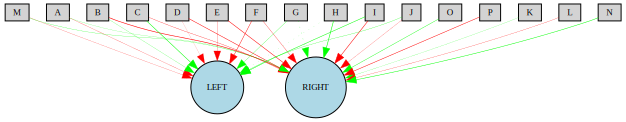
\includegraphics[width=0.86\linewidth]{img/network.PNG}
  \caption{Topology of the best individual.}
  \label{fig:ne_topology.}
\end{figure}

\section{Summary}

We have illustrated and analyzed the application of an evolutionary procedure to a virtual robotic agent with 2 similar evolutionary strategies. We showed how basic evolutionary algorithms (EA’s) and neuroevolution can emulate a Braitenberg vehicle in a way that it avoids obstacles. Both of the strategies satisfied the criteria of a Breitenberg-like obstacle avoidance vehicle. Through the evolutionary process we've evolved controllers that have a basic characteristic of autonomous agents that exhibited the ability to self-adjustment of their behavior in order to maximize its survival rate in a given environment. One example of the self-adjustment was seen in the case of wheel speed regulation. All these behaviors of the agents were not pre-designed but rather \emph{incorporated} in the scalar fitness function. The agent itself had to develop and optimize the right behavior by relying on set of fitness features aimed at developing straight navigation and obstacle avoidance behavior. In the first experiment, the results displayed that simple evolutionary algorithm is sufficient enough to evolve Brainanberg-like vehicle. With several experiments and by modifications of set parameters the evolved controllers displayed obstacle avoidance behavior. In contrast to a simple evolutionary algorithm, the experiments also proved that it is possible to evolve obstacle avoidance behavior using neuroevolution. However, we argue that the development of a simple obstacle avoidance behavior is an overhead using neuroevolution strategies for such a simple task. The evolution of an obstacle avoidance behavior with simple evolution algorithm has resulted in smart more lightweight efficient solutions.

Even though the project components and simple obstacle avoidance task, we have obtained great results and moreover experience in applying various evolution strategies. Our next work is aimed at evolving multimodal-behaviors on physical robotic agents in a mixed-reality environment.

\medskip

\newpage
\bibliographystyle{unsrt}
\bibliography{bibitems}

\end{document}
